\chapter{シス研ガチャ}
\begin{figure}
  \begin{center}
    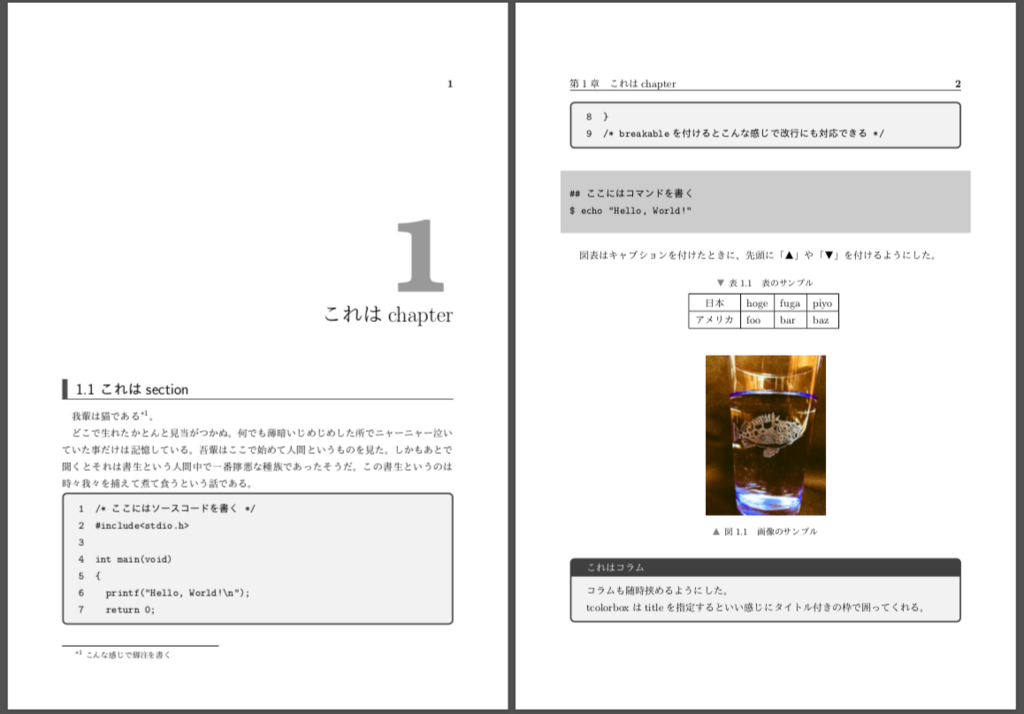
\includegraphics[width=5cm]{image/04-Intarasting/chap1/sample.png}
    \caption{シス研ガチャの画面}
    \label{syskengacha_top}
  \end{center}
\end{figure}
\section{はじめに}
こんにちわ.この章を担当するシステム工学研究会23卒OBのITO0oです.
長らくシス研でお世話になり,いろいろ感じで来たことがあります.
特に改善すべき点について述べ,それに対しての構想と試作の制作について述べます.
\section{シス研の課題}
私が感じていたシス研の課題点.それは,継続率の低さです.
実際にyyyy年からyyyy年での継続率はpp\%でした.
シス研はやることなすことは各人が自由に決めて行動してきました.
それ故に,目標の見つかる人,見つからない人に二分され,目標の見つからなかった人は幽霊部員となっていきました.
私はシス研で目標を見つけられた側でしたが,これは知り合った先輩や友人との関係がたまたまうまくいき,いろいろな経験ができたからこそであったと思っています.
ここで重要であるのが「人との関係性がたまたまうまくいった」というところです.
人間関係をうまく作るには以下のアプローチがあると思います.
\begin{quote}
  \begin{itemize}
    \item 1つ1つの関係の深化させる.
    \item 関係の数の増加させる.
  \end{itemize}
\end{quote}
OBという立場から言わせてもらうと前者は,かなりよい状態にあると思います.
実際に生き残ったシス研のOB同士のコミュニケーションはありますし,集まったりもします.
ということで,継続率の改善,ひいては後者のアプローチによる,シス研での人対人の交流の活発化が課題であると思っています.
せっかくシス研に目を着けてくれた学生さんには,是非ともシス研でよい学生生活を送っていただける方を少しでも増やしたいです.
そういった思いで次章から具体的な内容を述べていきます.
\section{解決策の構想}
\cite{izon}によると....以下が
\begin{quote}
  \begin{itemize}
    \item ちょっと手を伸ばせば届きそうな魅力的な報酬(目標)
    \item 
  \end{itemize}
\end{quote}
\section{システムの試作}
ここまでの内容では単なる自己啓発本的な内容になってしまうので技術本的な内容を混ぜていきます.
技術的な部分はそこまで詳しくないので,問題が起きたときの対処のきっかけになってくれたらいいなと思います.
\subsection{システム構成}
バックエンド部分については別に担当してくれた人がいるので,機会があれば詳しく書いてもらおうと思っています.
今は魔法で動いていると思っていてくれるとうれしいです.
\begin{figure}
  \begin{center}
    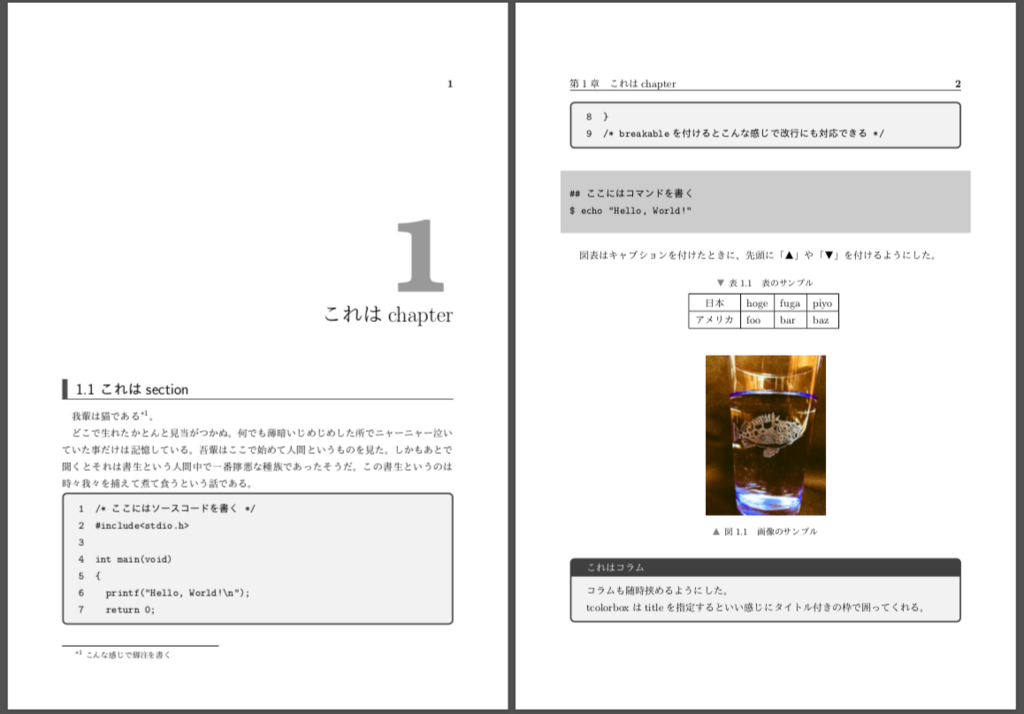
\includegraphics[width=5cm]{image/04-Intarasting/chap1/sample.png}
    \caption{シス研ガチャシステム構成}
    \label{syskengacha_system}
  \end{center}
\end{figure}
\subsection{制作過程でのハプニング}
ここの内容は題して「UnityでのWebアプリ制作初心者がハマりそうな沼」です.
Webアプリなのはとにかくユーザの敷居を低くしたかったからです.
ブラウザでできるのはかなり手軽ですよね.
ユーザは手軽である一方,これには初心者の制作側からするといくつか注意点があるというか,私がハマった沼があるのでその点について共有したいと思います.
他にも,Web開発初心者に向けたおまけ的なも盛り込んでおきます.
\subsubsection{フォント}
\subsubsection{非同期処理}
\subsubsection{Webサーバ}
\subsubsection{Github}
\subsubsection{画像のデータ形式}
\subsubsection{ガチャシステムのデータ形式}
\section{おわりに}
\begin{thebibliography}{9}
  \bibitem{izon} アダム・オルター,上原裕美子,"すべては依存症になるようデザインされている?――僕らをのめり込ませる6つのテクニック",DIAMOND online,\url{https://diamond.jp/articles/-/209526?page=2} (閲覧日 yyyy/mm/dd).
\end{thebibliography}